\section{Lab: File system}
\subsection{实验目的}
本实验旨在增进对操作系统的文件系统的了解。实验将会实现xv6系统对更大文件的支持,以及符号链接。目前 xv6 文件限制为 268 个块或 $268\times BSIZE$ 字节(xv6 中 BSIZE 为 1024)。这个限制是因为一个xv6 inode包含12个“直接”块号和一个“单间接”块号,这是指一个块最多可以容纳256个块号,总共$12+256=268$块。实验将更改 xv6 文件系统代码以支持每个 inode 中的“双间接”块,其中包含 256 个单间接块地址,每个块最多可包含 256 个数据块地址。结果将是一个文件最多可以包含 65803 个块,即 $256\times256+256+11$ 个块。
\subsection{实验步骤}
\subsubsection{实现Large files}
\begin{enumerate}
    \item 修改fs.h文件中的宏定义,改变文件系统块的结构。
          \begin{lstlisting}[language=c,title=修改fs.h宏定义]
    #define NDIRECT 11
    #define NINDIRECT (BSIZE / sizeof(uint))
    #define NDINDIRECT (NINDIRECT * NINDIRECT)
    #define MAXFILE (NDIRECT + NINDIRECT + NDINDIRECT)    
    \end{lstlisting}
    \item 修改fs.h中的dinode结构体,让addrs数组增加一个元素,以便储存二级索引块。
          \begin{lstlisting}[language=c,title=对dinode结构体的修改]
    struct dinode
    {
        short type;              // File type
        short major;             // Major device number (T_DEVICE only)
        short minor;             // Minor device number (T_DEVICE only)
        short nlink;             // Number of links to inode in file system
        uint size;               // Size of file (bytes)
        uint addrs[NDIRECT + 2]; // Data block addresses
    };    
    \end{lstlisting}
    \item 修改file.h中的inode结构体,修改方式同上。
          \begin{lstlisting}[language=c,title=对inode结构体的修改]
    // in-memory copy of an inode
    struct inode
    {
        uint dev;              // Device number
        uint inum;             // Inode number
        int ref;               // Reference count
        struct sleeplock lock; // protects everything below here
        int valid;             // inode has been read from disk?
    
        short type; // copy of disk inode
        short major;
        short minor;
        short nlink;
        uint size;
        uint addrs[NDIRECT + 2];
    };    
    \end{lstlisting}
    \item 修改fs.c文件中的bmap函数,增加对二级索引块的处理。
          \begin{lstlisting}[language=c,title=对bmap函数的修改]
    static uint bmap(struct inode *ip, uint bn)
    {
        uint addr, *a;
        struct buf *bp;
    
        ...
    
        // 二级索引块处理
        if (bn < NDINDIRECT)
        {
            // 检查二级间接块的起始地址是否已分配,如果未分配则分配一个新的块
            if ((addr = ip->addrs[NDIRECT + 1]) == 0)
                ip->addrs[NDIRECT + 1] = addr = balloc(ip->dev);
        
            // 读取二级间接块的数据
            bp = bread(ip->dev, addr);
            a = (uint *)bp->data;
        
            // 获取一级间接块地址,如果未分配则分配一个新的块
            if ((addr = a[bn / NINDIRECT]) == 0)
            {
                a[bn / NINDIRECT] = addr = balloc(ip->dev);
                log_write(bp);
            }
            brelse(bp);
        
            // 读取一级间接块的数据
            bp = bread(ip->dev, addr);
            a = (uint *)bp->data;
        
            // 获取最终的目标块地址,如果未分配则分配一个新的块
            if ((addr = a[bn % NINDIRECT]) == 0)
            {
                a[bn % NINDIRECT] = addr = balloc(ip->dev);
                log_write(bp);
            }
            brelse(bp);
            return addr;
        }
    
        // 如果块号超出范围,触发panic
        panic("bmap: out of range");
    }    
    \end{lstlisting}
    \item 修改fs.c文件中的itrunc函数,增加对二级索引块的处理。
          \begin{lstlisting}[language=c,title=对itrunc函数的修改]
    void itrunc(struct inode *ip)
    {
        int i, j;
        struct buf *bp, *bp2;
        uint *a, *a2;
    
        ...
    
        // 处理二级间接块
        if (ip->addrs[NDIRECT + 1])
        {
            // 读取二级间接块
            bp = bread(ip->dev, ip->addrs[NDIRECT + 1]);
            a = (uint *)bp->data;
        
            // 释放二级间接块中的每个一级间接块
            for (j = 0; j < NINDIRECT; j++)
            {
                if (a[j])
                {
                    // 读取一级间接块
                    bp2 = bread(ip->dev, a[j]);
                    a2 = (uint *)bp2->data;
            
                    // 释放一级间接块中的每个块
                    for (i = 0; i < NINDIRECT; i++)
                    {
                        if (a2[i])
                        bfree(ip->dev, a2[i]);
                    }
                    brelse(bp2);
            
                    // 释放一级间接块本身
                    bfree(ip->dev, a[j]);
                    a[j] = 0;
                }
            }
            brelse(bp);
        
            // 释放二级间接块本身
            bfree(ip->dev, ip->addrs[NDIRECT + 1]);
            ip->addrs[NDIRECT + 1] = 0;
        }
    
        // 重置inode大小并更新inode信息
        ip->size = 0;
        iupdate(ip);
    }    
    \end{lstlisting}
\end{enumerate}

\subsubsection{实现Symbolic links}
符号链接(Symbolic Link,简称symlink)是一种文件系统对象,它是一种特殊类型的文件,指向另一个文件或目录。符号链接本质上是一个包含指向目标文件或目录路径的文本文件。它允许用户在文件系统中创建一个指向另一个文件或目录的快捷方式。

\begin{enumerate}
    \item 仿照之前的方式,注册一个名为symlink的系统调用。
    \item 在stat.h中增加一个宏,表示符号链接。
          \begin{lstlisting}[language=c,title=添加表示符号链接的文件类型]
    #define T_SYMLINK 4 // Symbolic link    
    \end{lstlisting}
    \item 在fcntl.h中添加一个宏,表示不跟随符号链接的文件打开模式。
          \begin{lstlisting}[language=c,title=添加不跟随符号链接的文件打开模式的宏]
    #define O_NOFOLLOW 0x800
    \end{lstlisting}
    \item 在sysfile.c文件中实现符号链接的系统调用
          \begin{lstlisting}[language=c,title=sys\_symlink的实现]
    uint64 sys_symlink(void)
    {
        // 定义用于存储目标路径和符号链接路径的字符数组
        char target[MAXPATH], path[MAXPATH]; 
    
        // 获取符号链接指向的目标路径和符号链接路径
        // 如果获取参数失败,则返回-1
        if (argstr(0, target, MAXPATH) < 0 
        || argstr(1, path, MAXPATH) < 0)
        return -1;
    
        begin_op();       // 开始文件系统操作
        struct inode *ip; // 定义inode结构指针
    
        // 创建一个类型为符号链接的inode,路径为`path`
        // 如果创建失败,结束操作并返回-1
        if ((ip = create(path, T_SYMLINK, 0, 0)) == 0)
        {
            end_op();
            return -1;
        }
    
        // 将目标路径写入到符号链接的inode中
        // 如果写入的字节数少于MAXPATH,解锁并释放inode,然后结束操作返回-1
        if (writei(ip, 0, (uint64)target, 0, MAXPATH) < MAXPATH)
        {
            iunlockput(ip);
            end_op();
            return -1;
        }
    
        iunlockput(ip); // 解锁并释放inode
        end_op();       // 结束文件系统操作
        return 0;       // 返回0表示成功
    }    
    \end{lstlisting}
    \item 修改sysfile.c文件中的sys\_open系统调用,增加符号链接的打开方法。
          \begin{lstlisting}[language=c,title=对sys\_open函数的修改]
    uint64 sys_open(void)
    {
        char path[MAXPATH]; // 用于存储文件路径的字符数组
        int fd, omode;      // fd表示文件描述符,omode表示文件打开模式
        struct file *f;     // 文件结构指针
        struct inode *ip;   // inode结构指针
        int n;              // 临时变量,用于存储函数返回值
    
        ...
    
        // 处理符号链接,逐层解析直到达到实际文件或达到限制
        int layer = 0; // 跟踪符号链接的层数
        while (ip->type == T_SYMLINK && !(omode & O_NOFOLLOW))
        {
            layer++;                // 增加层数
            if (layer == THRESHOLD) // 如果层数达到阈值,返回错误
            {
                iunlockput(ip); // 解锁并释放inode
                end_op();       // 结束操作
                return -1;
            }
            else // 继续解析符号链接
            {
                // 读取符号链接指向的路径
                if (readi(ip, 0, (uint64)path, 0, MAXPATH) < MAXPATH)
                {
                    iunlockput(ip); // 如果读取失败,解锁并释放inode
                    end_op();       // 结束操作
                    return -1;
                }
                iunlockput(ip);   // 解锁并释放当前符号链接的inode
                ip = namei(path); // 解析符号链接指向的路径
                if (ip == 0)
                {
                    end_op(); // 如果解析失败,结束操作并返回-1
                    return -1;
                }
                ilock(ip); // 锁定解析后的inode
            }
        }
    
        ...
    
        return fd; // 返回文件描述符
    }    
    \end{lstlisting}
\end{enumerate}

\subsection{评测结果}
利用grade-lab-fs脚本评测,得到结果如图\ref{fig:fs}。
\begin{figure}[ht]
    \centering
    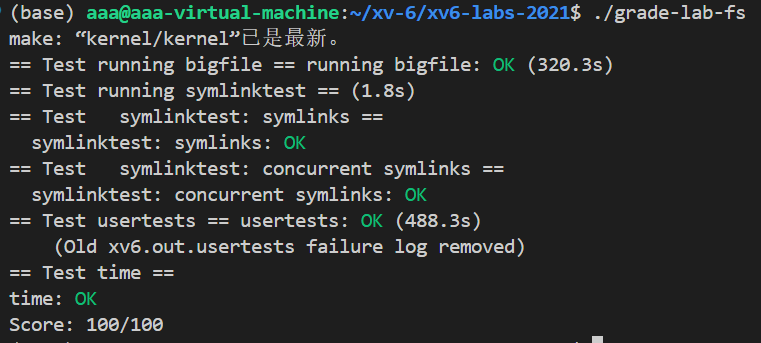
\includegraphics[width=\linewidth]{pics/fs评测结果.png}
    \caption{评测结果}
    \label{fig:fs}
\end{figure}
\subsection{实验小结}


实验完成后,我成功地为xv6文件系统增加了对大文件的支持,并实现了符号链接的功能。

在实现大文件支持时,我通过修改文件系统的块结构,引入了“双间接”块的概念,使得一个文件能够支持多达65803个块。这大幅提高了xv6系统能够处理的文件大小限制。实现过程中,我深刻理解了文件系统块管理的机制,特别是间接块的使用与管理。

符号链接的实现则为xv6文件系统增加了文件引用的灵活性。此部分实验帮助我理解了符号链接在文件系统中的作用及其实现原理。

通过对以上两个功能的实现和测试,我加深了对文件系统的理解,尤其是在文件存储结构和文件引用管理方面的知识。实验结果表明,所有功能均按预期工作,为日后深入研究和开发复杂的文件系统奠定了基础。